\documentclass[journal]{IEEEtran}
\usepackage{cite}
\usepackage{amsmath,amssymb}
\usepackage{booktabs}
\usepackage{graphicx}
\usepackage{multirow}
\usepackage{tikz}
\usetikzlibrary{positioning,arrows.meta,fit,calc}
\usepackage{microtype}
\usepackage[hidelinks]{hyperref}

\title{Improving Digital Forensic Triage in Network-Based Anomaly Detection Systems: An Explainable Anomaly Detection Approach for Transparency, Reliability, and Investigator Decision-Making}
\author{Damilola~Popoola}

\begin{document}
\maketitle

\begin{abstract}
In a forensic investigation an anomaly score is not evidence: the investigator must still decide which alerts to examine first and must later be able to justify that decision. We present \textsc{XTriage}, a framework that turns the alerts of an unsupervised network detector into documented triage decisions. Each alert is explained with exact TreeSHAP, encoded with its traffic values and score band, and prioritized by an ordered rule list learned from investigator decisions; a disagreement guard flags decisions the rules should not be trusted with, and every decision is written to a hash-chained, replayable ledger. We evaluate the framework as a forensic tool on CIC-IDS2017, NF-UNSW-NB15-v3, and NF-CSE-CIC-IDS2018-v3 over ten seeds, measuring examination workload, the rate at which severe events are dismissed without warning, explanation stability, and reproducibility. Rule-based triage ranks severe events higher than score-only ranking on all three corpora, every audited decision was replayed exactly, tampering was detected at the altered record, and the guard cut silent dismissals of severe events from 28\% to 7\% on CIC-IDS2017. We also report eight limitations: explanations change when the detector is retrained (top-5 agreement 0.27--0.51), a port change flips the triage tier of 36\% of attacks without changing their score, and triage rules do not transfer between networks. We release \textsc{XFT-Bench}, the explained-triage data behind these results.
\end{abstract}

\begin{IEEEkeywords}
Digital forensics, forensic triage, network anomaly detection, explainable AI, SHAP, rule induction, chain of custody.
\end{IEEEkeywords}

% ---------------------------------------------------------------------------
\section{Introduction}
\label{sec:intro}
Digital forensic investigations increasingly depend on large volumes of network traffic, system logs, and security alerts. Before a complete examination can begin, investigators perform \emph{triage}: the rapid identification and prioritization of the items most likely to contain relevant evidence \cite{rogers}. Network traffic is a recognized forensic source in incident response \cite{nist}, and anomaly detectors can point investigators to traffic that deviates from normal behaviour, including activity that matches no known signature \cite{iforest}. Their practical value, however, is limited when they produce many alerts, many false positives, and scores without reasons.

Alert volume (C1) overwhelms analysts, most of whose alarms are false positives \cite{alahmadi}. The score is opaque (C2): it shows \emph{that} a flow is unusual but not \emph{why} \cite{sommer}. Without stated reasons, prioritization depends on the analyst and becomes inconsistent (C3). Accountability suffers (C4): forensic practice requires that the steps to a conclusion are documented, reproducible, and open to independent scrutiny \cite{nist,iso27042}. Underneath lies model reliability (C5): benchmarks contain labelling errors \cite{engelen}, detectors may rely on shortcut features \cite{trustee,arp}, and accuracy can degrade silently as traffic drifts.

The central problem is therefore not detection but turning a model output into a transparent, reliable, and investigator-usable triage decision. In \textsc{XTriage}, SHAP explains each alert \cite{shap}; because attributions alone are too technical and too variable to act on \cite{warnecke}, induced IF--THEN rules turn recurring combinations of traffic values, attributions, and scores into consistent priorities; and every decision is recorded so that an examiner can reconstruct and justify it. Explanations must be \emph{faithful} to the detector (R1) and \emph{stable} (R2); decisions must be \emph{actionable} (R3) and \emph{auditable} from preserved inputs (R4); and the investigator must stay \emph{in the loop}, with the tool's uncertainty visible (R5).

This paper contributes (i)~\textsc{XTriage}, which combines exact attributions, explanation-augmented rules, a disagreement guard, and a hash-chained, replayable triage record (Section~\ref{sec:method}); (ii)~an evaluation protocol that judges explainable detection by forensic criteria, namely examination workload, a \emph{known error rate} of severe events dismissed without warning, explanation reproducibility, and decision replay, applied to three corpora with ten seeds (Sections~\ref{sec:eval}--\ref{sec:results}); (iii)~eight limitations of explainable triage, each with its forensic consequence and a tested mitigation (Section~\ref{sec:limits}); and (iv)~\textsc{XFT-Bench}, an explained-triage dataset for comparing these properties across studies (Section~\ref{sec:bench}).

% ---------------------------------------------------------------------------
\section{Background and Related Work}
\label{sec:related}

\emph{Forensic triage and validation.} Rogers et al.\ \cite{rogers} formalized triage as a pre-examination step that identifies the most promising evidence quickly, before a full laboratory examination. NIST SP~800-86 \cite{nist} integrates network data into incident-response forensics, ISO/IEC~27037 \cite{iso27037} governs the preservation of digital evidence, and ISO/IEC~27042 \cite{iso27042} requires analysis methods to be fit for purpose, repeatable, and recorded in enough detail for independent scrutiny. Admissibility tests such as \emph{Daubert} \cite{daubert} ask whether a method has been tested and whether its error rate is known. An automated triage tool must therefore be judged not only by accuracy, but also by whether its decisions can be reproduced and by how often it discards relevant evidence.

\emph{Explaining network detectors.} Anomaly detection uses isolation forests \cite{iforest} or autoencoders \cite{kitsune}; supervised boosted trees \cite{xgboost} are more accurate on labelled benchmarks but miss unseen attack classes. SHAP \cite{shap} attributes a prediction to its features, exactly for tree ensembles \cite{treeshap}, and LIME \cite{lime} fits local surrogates; both have been applied to forensic intrusion analysis \cite{hermosilla}. Their trustworthiness is contested: methods differ in accuracy and stability \cite{warnecke}, SHAP explanations are unstable across retraining \cite{maseno}, and explanations can be manipulated \cite{fooling}. Gombar \cite{gombar} ranked flows by confidence, SHAP strength, and severity.

\emph{Rules.} RIPPER \cite{ripper} learns compact rule lists and Anchors \cite{anchors} high-precision local rules. Trustee \cite{trustee} extracted trees from detectors to expose shortcuts, Adewole et al.\ \cite{adewole} explained an IoT detector with induced rules, and Rudin \cite{rudin} argues for interpretable models in high-stakes settings. Our prior work on DER networks attached decision paths to alerts \cite{cysider}, flagged alerts whose SHAP values and rules disagree \cite{excyder}, and combined both for threat reasoning \cite{cytrex}; SOC practice also calls for rules rather than opaque scores \cite{gridsoc}.

As Table~\ref{tab:compare} shows, stability audits \cite{maseno,warnecke} and SHAP-based ranking \cite{gombar} exist separately and for supervised classifiers. No prior work learns triage rules \emph{from} the explanations, measures workload, fidelity, and stability on the same alerts, records decisions in replayable form, or releases the explanations as a benchmark.

\begin{table}[t]
\centering
\caption{Comparison With Representative Prior Work ($\circ$ = Partial)}
\label{tab:compare}
\setlength{\tabcolsep}{3pt}
\footnotesize
\begin{tabular}{@{}lccccc@{}}
\toprule
     & Local &       & Stability & Triage & Audit\\
Work & attr. & Rules & eval.     & metric & record\\
\midrule
Hermosilla et al. \cite{hermosilla} & \checkmark & --         & --         & -- & -- \\
Warnecke, Maseno \cite{warnecke,maseno} & \checkmark & --         & \checkmark & -- & -- \\
Trustee, Adewole \cite{trustee,adewole} & --     & \checkmark & --         & -- & -- \\
Gombar \cite{gombar}             & \checkmark & --         & --         & $\circ$ & -- \\
ExCyDER \cite{excyder}           & \checkmark & \checkmark & $\circ$    & -- & -- \\
CyTReX \cite{cytrex}             & \checkmark & \checkmark & --         & $\circ$ & $\circ$ \\
This work                        & \checkmark & \checkmark & \checkmark & \checkmark & \checkmark \\
\bottomrule
\end{tabular}
\end{table}

% ---------------------------------------------------------------------------
\begin{figure*}[t]
\centering
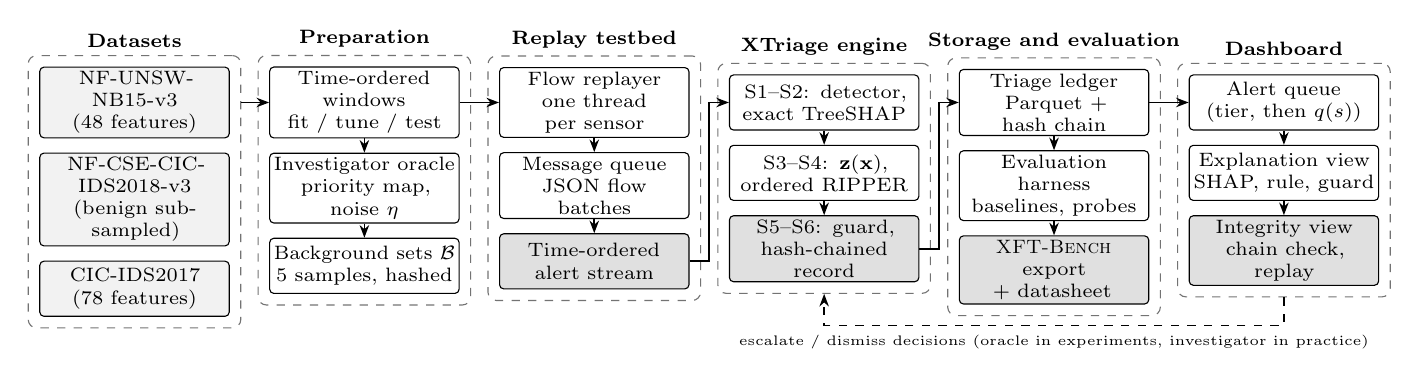
\begin{tikzpicture}[
  font=\scriptsize,
  box/.style={draw, rounded corners=1.5pt, align=center, text width=23mm, minimum height=7mm, inner sep=1.5pt, fill=white},
  data/.style={box, fill=black!5},
  hot/.style={box, fill=black!12},
  panel/.style={draw=black!55, dashed, rounded corners=3pt, inner sep=1.4mm},
  ptitle/.style={font=\scriptsize\bfseries, inner sep=1pt},
  arr/.style={-{Stealth[length=1.6mm]}, semithick},
  fb/.style={-{Stealth[length=1.6mm]}, semithick, dashed}]
\node[data] (d1) {NF-UNSW-NB15-v3\\(48 features)};
\node[data, below=1.8mm of d1] (d2) {NF-CSE-CIC-IDS2018-v3\\(benign subsampled)};
\node[data, below=1.8mm of d2] (d3) {CIC-IDS2017\\(78 features)};
\node[box, right=5mm of d1] (split) {Time-ordered windows\\fit / tune / test};
\node[box, below=1.8mm of split] (oracle) {Investigator oracle\\priority map, noise $\eta$};
\node[box, below=1.8mm of oracle] (bgs) {Background sets $\mathcal{B}$\\5 samples, hashed};
\node[box, right=5mm of split] (replay) {Flow replayer\\one thread per sensor};
\node[box, below=1.8mm of replay] (queue) {Message queue\\JSON flow batches};
\node[hot, below=1.8mm of queue] (stream) {Time-ordered\\alert stream};
\node[box, right=5mm of replay] (e1) {S1--S2: detector,\\exact TreeSHAP};
\node[box, below=1.8mm of e1] (e2) {S3--S4: $\mathbf{z}(\mathbf{x})$,\\ordered RIPPER};
\node[hot, below=1.8mm of e2] (e3) {S5--S6: guard,\\hash-chained record};
\node[box, right=5mm of e1] (ledger) {Triage ledger\\Parquet + hash chain};
\node[box, below=1.8mm of ledger] (harness) {Evaluation harness\\baselines, probes};
\node[hot, below=1.8mm of harness] (bench) {\textsc{XFT-Bench} export\\+ datasheet};
\node[box, right=5mm of ledger] (v1) {Alert queue\\(tier, then $q(s)$)};
\node[box, below=1.8mm of v1] (v2) {Explanation view\\SHAP, rule, guard};
\node[hot, below=1.8mm of v2] (v3) {Integrity view\\chain check, replay};
\node[panel, fit=(d1)(d3)] (P1) {};
\node[panel, fit=(split)(bgs)] (P2) {};
\node[panel, fit=(replay)(stream)] (P3) {};
\node[panel, fit=(e1)(e3)] (P4) {};
\node[panel, fit=(ledger)(bench)] (P5) {};
\node[panel, fit=(v1)(v3)] (P6) {};
\node[ptitle, above=0.5mm of P1.north] {Datasets};
\node[ptitle, above=0.5mm of P2.north] {Preparation};
\node[ptitle, above=0.5mm of P3.north] {Replay testbed};
\node[ptitle, above=0.5mm of P4.north] {\textsc{XTriage} engine};
\node[ptitle, above=0.5mm of P5.north] {Storage and evaluation};
\node[ptitle, above=0.5mm of P6.north] {Dashboard};
\draw[arr] (P1.east |- split.west) -- (split.west);
\draw[arr] (split) -- (oracle);
\draw[arr] (oracle) -- (bgs);
\draw[arr] (split.east) -- (replay.west);
\draw[arr] (replay) -- (queue);
\draw[arr] (queue) -- (stream);
\draw[arr] (stream.east) -- ++(2.5mm,0) |- (e1.west);
\draw[arr] (e1) -- (e2);
\draw[arr] (e2) -- (e3);
\draw[arr] (e3.east) -- ++(2.5mm,0) |- (ledger.west);
\draw[arr] (ledger) -- (harness);
\draw[arr] (harness) -- (bench);
\draw[arr] (ledger.east) -- (v1.west);
\draw[arr] (v1) -- (v2);
\draw[arr] (v2) -- (v3);
\coordinate (yb) at ($(P4.south)+(0,-4mm)$);
\draw[fb] (P6.south) -- (P6.south |- yb) -- node[below, font=\tiny]{escalate / dismiss decisions (oracle in experiments, investigator in practice)} (P4.south |- yb) -- (P4.south);
\end{tikzpicture}
\caption{\textsc{XTriage} and its evaluation. Flow corpora are cut into time-ordered windows, replayed by sensor threads, and processed by the engine stages S1--S6. Every decision is appended to a hash-chained ledger that feeds the evaluation harness, the \textsc{XFT-Bench} export, and a Streamlit dashboard. The dashed arrow returns decisions, which come from the oracle in the experiments.}
\label{fig:pipeline}
\end{figure*}

\section{The \textsc{XTriage} Framework}
\label{sec:method}
Fig.~\ref{fig:pipeline} shows the framework and its evaluation setting. Each flow is a feature vector $\mathbf{x}\in\mathbb{R}^d$. Identifiers (addresses, source port, timestamps, flow IDs) are kept in the record but excluded from the model input, so no stage can learn shortcuts from them; undefined values are set to $-1$.

\subsection{S1: Anomaly Detection}
The primary detector is an isolation forest \cite{iforest} (100 trees, 256 samples per tree) trained on 100{,}000 benign flows from the earliest time window. It never sees attack labels. We use the score $s(\mathbf{x})=-\mathbb{E}[h(\mathbf{x})]$, the negative mean isolation depth, which is a strictly monotone transform of the usual anomaly score and keeps attributions exact (S2). The score is mapped to a percentile $q(s)\in[0,1]$, the empirical distribution function over 50{,}000 held-out benign calibration flows, so that a threshold has the same meaning on every corpus. A flow becomes an alert when $q(s)\geq\theta=0.95$. An autoencoder (reconstruction error) and supervised XGBoost \cite{xgboost} serve as alternative detectors.

\subsection{S2: Event-Level Attribution (R1)}
For every alert, SHAP splits the score into feature contributions,
\begin{equation}
s(\mathbf{x})=\phi_0+\textstyle\sum_{j=1}^{d}\phi_j(\mathbf{x}),
\end{equation}
where $\phi_0$ is the expected score over a background set $\mathcal{B}$ of 100 benign flows from the fit window. For the isolation forest we use interventional TreeSHAP \cite{treeshap}, which is exact; additivity holds to $10^{-6}$ in our tests. The autoencoder uses KernelSHAP, and LIME \cite{lime} serves as a comparison. Because attributions depend on $\mathcal{B}$, the SHA-256 hash of $\mathcal{B}$ is stored with every decision. $T_k(\mathbf{x})$ denotes the $k=5$ features with the largest $|\phi_j|$.

\subsection{S3: SHAP-Augmented Representation}
Raw SHAP vectors are too detailed for consistent decisions, and raw-feature rules can rely on patterns the detector ignores, so each alert is encoded as
\begin{equation}
\mathbf{z}(\mathbf{x})=\big[\,\mathrm{disc}(\mathbf{x}),\;\pi_1(\mathbf{x}),\dots,\pi_d(\mathbf{x}),\;\mathrm{band}(q)\,\big],
\end{equation}
where $\mathrm{disc}$ assigns each feature to one of five quantile bins fitted on the fit window; $\pi_j(\mathbf{x})=\mathbb{1}[\,j\in T_k(\mathbf{x})\wedge\phi_j(\mathbf{x})>0\,]$ is true when feature $j$ is among the main reasons the flow looked anomalous; and $\mathrm{band}(q)$ is \emph{low} for $q<0.99$, \emph{medium} for $q<0.999$, and \emph{high} otherwise. A rule can then combine what the traffic looked like with why the detector reacted, e.g., \textsf{IF band=high AND $\pi_{\text{dst\_port}}$ AND out\_bytes$\,\in\,$Q5 THEN P1}.

\subsection{S4: Rule Induction (R3)}
Each alert receives a priority $p\in\{\text{P1},\text{P2},\text{P3}\}$: escalate, review, or dismiss. Rules are learned from investigator decisions on the middle (tune) window, so the framework is semi-supervised: the detector never sees labels, but the triage layer learns from confirmed decisions, as in an operational SOC. RIPPER \cite{ripper} is binary, so we apply it as an ordered list in the style of JRip: classes are learned from rarest to most frequent, each against the remaining ones, and the most frequent class becomes the default (catch-all) rule. Rules have at most four conditions and each class at most 40 rules, and training uses a class-stratified sample of at most 15{,}000 alerts. Each rule set is versioned and stored with the support and precision of every rule. A depth-limited tree surrogate \cite{trustee} and Anchors \cite{anchors} serve as alternatives.

\subsection{S5: Disagreement Guard (R5)}
Rules simplify the detector, and the simplification can be wrong. Extending the per-alert verification of \cite{excyder} from explanations to decisions, the guard marks a decision \emph{contested} when (i)~only the default rule fired, (ii)~a P3 rule fired although $q\geq 0.99$, or (iii)~a P1 rule fired in the low band. Our Phase~2 design sent every contested case to review (P2), which \emph{demotes} true P1 events whenever an escalation rule meets a low score. The guard therefore may only \emph{raise} attention: contested P2/P3 decisions become P2, and contested P1 decisions stay P1 and are flagged; the Phase~2 rule is kept as an ablation. A \emph{calibrated} variant replaces (i)--(ii) by an estimated risk: for each (rule, band) cell, the tune window gives the smoothed share of P1 events among the alerts the cell did not escalate, $(n_{\text{P1}}+a\bar{p})/(n+a)$ with prior $\bar{p}$ and $a=20$, and the cell is contested when the share reaches $\tau=0.01$. The queue is ordered by tier, then $q$, then $s$ (to break ties where $q$ saturates).

\subsection{S6: Forensic Triage Record (R4)}
Each decision is appended as a record $r_i$ holding the flow identifiers and features; $s$, $q$, and $\boldsymbol{\phi}$; the hash of $\mathcal{B}$; the fired rule and its text; the content hashes of the detector, background set, and rule set; the guard status and reason; a timestamp; and the investigator response. Records are serialized canonically (sorted-key JSON) and chained as $h_i=\mathrm{SHA256}(h_{i-1}\,\|\,r_i)$ in append-only Parquet parts. Verification recomputes the chain and reports the first altered record; replay loads the versioned artifacts named in a record and recomputes $s$, $q$, $\boldsymbol{\phi}$, the rule, and the tier, so any decision can be reconstructed from its preserved inputs \cite{nist,iso27042}. Investigator responses update the rules only after confirmation against evidence, and each re-learned rule set must pass a frozen test window. The implementation uses Python, scikit-learn, \texttt{shap}, \texttt{wittgenstein}, and PyArrow, with a streaming testbed and a Streamlit dashboard.

% ---------------------------------------------------------------------------
\section{Evaluation Design}
\label{sec:eval}
We evaluate \textsc{XTriage} as a forensic tool, asking what a method validation \cite{iso27042,daubert} would ask: does it reduce examination effort, how often does it dismiss a severe event without warning, are its explanations reproducible, and can each decision be reconstructed?

\subsection{Datasets, Splits, and Oracle}
Table~\ref{tab:data} lists the corpora. The NetFlow~v3 corpora \cite{nfv3,unsw} share one feature set, which allows a cross-corpus test; CIC-IDS2017 \cite{cicids} (original release) links to prior work. For NF-CSE-CIC-IDS2018-v3 we keep a deterministic 10\% of benign rows and every attack row. Splits follow time \cite{arp}: the detector, calibration flows, and $\mathcal{B}$ come from the earliest window, rules from the middle (tune) window, and all metrics from the last (test) window. In the two CIC corpora each attack occupies one block of one day, so after an early benign-heavy fit window the traffic is cut into 20- or 30-minute blocks that alternate between tune and test; some classes still occur on one side only, which tests unseen classes. Tune and test windows are sampled (benign 10--15\%, at most 15{,}000 flows per class).

Real analysts' decisions are not available for these corpora, so a documented \emph{oracle} maps attack classes to priorities by likely impact: code execution, persistence, and covert control to P1 (Table~\ref{tab:data}); reconnaissance, fuzzing, brute force, and DoS to P2; benign to P3. A fraction $\eta\in\{0,0.1,0.2,0.3\}$ of labels is flipped to simulate analyst error.

\begin{table}[t]
\centering
\caption{Corpora (Test Window After Sampling)}
\label{tab:data}
\setlength{\tabcolsep}{2.5pt}
\footnotesize
\begin{tabular}{@{}lccc@{}}
\toprule
 & NF-UNSW-NB15 & NF-CIC-IDS2018 & CIC-IDS2017\\
\midrule
Flows (used)    & 2.37M & 20.1M (4.35M) & 2.83M\\
Features        & 48 & 48 & 78\\
Split           & time 40/30/30 & 30-min blocks & 20-min blocks\\
Test flows      & 152{,}024 & 134{,}151 & 149{,}837\\
Test P1 flows   & 17{,}455 & 30{,}241 & 963\\
P1 classes      & \parbox[t]{17mm}{\centering Exploits, Back-\\door, Shellcode,\\Worms} & \parbox[t]{17mm}{\centering Bot, Infiltration,\\SQL injection} & \parbox[t]{17mm}{\centering Bot, Infiltration,\\Heartbleed,\\SQL injection}\\
\bottomrule
\end{tabular}
\end{table}

\subsection{Metrics}
Let $A$ be the test alerts in queue order and $A_1\subseteq A$ the alerts whose oracle priority is P1.
\begin{itemize}
\item \emph{Workload@90} (effort, lower is better): the share of $A$ an investigator must examine, in queue order, to find 90\% of $A_1$.
\item \emph{Recall@$b$} and \emph{NDCG}: the share of all test P1 flows found in the first $b$ alerts, and normalized discounted cumulative gain with relevance 2/1/0 for P1/P2/P3.
\item \emph{Silent dismissal rate} (known error rate, lower is better): the share of $A_1$ that a rule dismissed (P3) without the guard contesting it. These are severe events the tool discards with no visible doubt.
\item \emph{Rule quality}: P1-F1 and macro-F1 of the final tier against the oracle; \emph{fidelity}, the share of features a fired rule references positively that lie in $T_5(\mathbf{x})$; number and length of rules.
\item \emph{Explanation reliability}: top-5 Jaccard and Kendall's $\tau$ between attributions of 600 stratified alerts under different backgrounds or detector seeds; deletion AUC, the normalized score as top-ranked features are replaced by background values (lower is more faithful).
\item \emph{Accountability}: replay success, tamper detection, record size, and latency.
\end{itemize}

\subsection{Baselines, Ablations, and Probes}
B1 ranks alerts by score only; B2 is supervised XGBoost with SHAP; B3 learns RIPPER on raw-feature bins without predicates, band, or guard \cite{rudin}; B4 is a tree surrogate \cite{trustee}; B5 substitutes LIME for SHAP; Anchors explains alerts one at a time. Ablations remove the predicates, the band, or the guard, or use the Phase~2 guard. Probes vary the background set (size 10--500, window, traffic mix), remove suspected shortcut features, compare early and late test halves, test across corpora, perturb attacker-controllable features (padding, timing, port, within protocol limits; no traffic is generated), and sweep $\eta$, $\theta$, $\tau$, and the forest size.

\subsection{Testbed and Protocol}
The testbed replays a test window as a stream: four sensor threads publish 60{,}000 flows in time order as JSON batches to a queue, the engine consumes them, and a writer appends records to the ledger. Main results use ten seeds; each method is compared with \textsc{XTriage} by paired two-sided Wilcoxon signed-rank tests at $\alpha=0.05$. Probes use one to three seeds, and KernelSHAP, LIME, and Anchors run on stratified samples of 1{,}500--3{,}000 alerts.

% ---------------------------------------------------------------------------
\section{Results}
\label{sec:results}

\begin{table*}[t]
\centering
\caption{Triage Results, Mean Over Ten Seeds. W = Workload@90 ($\downarrow$), N = NDCG ($\uparrow$), F = P1-F1 ($\uparrow$), S = Silent Dismissals in \% of Alerted P1 Events ($\downarrow$). $^{*}$: Differs From \textsc{XTriage} (Wilcoxon, $p<0.05$). B2 Is Supervised and Alerts on 59--66k Flows.}
\label{tab:main}
\setlength{\tabcolsep}{4.5pt}
\scriptsize
\begin{tabular}{@{}l cccc c cccc c cccc@{}}
\toprule
& \multicolumn{4}{c}{NF-UNSW-NB15} && \multicolumn{4}{c}{NF-CIC-IDS2018} && \multicolumn{4}{c}{CIC-IDS2017}\\
\cmidrule{2-5}\cmidrule{7-10}\cmidrule{12-15}
Method & W & N & F & S && W & N & F & S && W & N & F & S\\
\midrule
B1 score only            & 0.93$^{*}$ & 0.82$^{*}$ & -- & -- && 0.86 & 0.81$^{*}$ & -- & -- && 0.50$^{*}$ & 0.92$^{*}$ & -- & --\\
B2 XGBoost + SHAP        & 0.83$^{*}$ & 0.95$^{*}$ & -- & -- && 0.89$^{*}$ & 0.95$^{*}$ & -- & -- && 0.88$^{*}$ & 0.98$^{*}$ & -- & --\\
B3 raw-feature rules     & 0.41$^{*}$ & 0.97$^{*}$ & 0.74 & 0.1$^{*}$ && 0.83 & 0.84 & 0.28 & 14.3 && 0.54$^{*}$ & 0.99$^{*}$ & 0.79 & 26.0$^{*}$\\
B4 tree surrogate        & 0.49$^{*}$ & 0.96$^{*}$ & 0.71$^{*}$ & 0.3$^{*}$ && 0.89$^{*}$ & 0.84 & 0.03$^{*}$ & 40.4$^{*}$ && 0.78$^{*}$ & 0.95$^{*}$ & 0.47$^{*}$ & 20.3$^{*}$\\
\textbf{\textsc{XTriage}} & 0.85 & 0.94 & 0.74 & 0.0 && 0.81 & 0.84 & 0.29 & 15.0 && 0.21 & 0.95 & 0.75 & 7.2\\
\midrule
$-$ SHAP predicates      & 0.84 & 0.94 & 0.75 & 0.0 && 0.82 & 0.84 & 0.28 & 13.0 && 0.20 & 0.95 & 0.79 & 7.1\\
$-$ score band           & 0.85 & 0.94 & 0.74 & 0.0 && 0.79 & 0.84 & 0.29 & 14.3 && 0.20 & 0.95 & 0.75 & 6.0\\
$-$ guard                & 0.42$^{*}$ & 0.97$^{*}$ & 0.74 & 0.1$^{*}$ && 0.81 & 0.84$^{*}$ & 0.29 & 17.0$^{*}$ && 0.54$^{*}$ & 0.99$^{*}$ & 0.75 & 28.1$^{*}$\\
Phase~2 guard (review)   & 0.93$^{*}$ & 0.84$^{*}$ & 0.06$^{*}$ & 0.0 && 0.84 & 0.84 & 0.22 & 15.0 && 0.50$^{*}$ & 0.94$^{*}$ & 0.53$^{*}$ & 7.2\\
\midrule
Calibrated guard         & 0.43$^{*}$ & 0.97$^{*}$ & 0.74 & 0.1$^{*}$ && 0.56$^{*}$ & 0.83$^{*}$ & 0.29 & 0.2$^{*}$ && 0.54$^{*}$ & 0.99$^{*}$ & 0.75 & 28.1$^{*}$\\
SHAP-gated bins          & 0.91$^{*}$ & 0.90$^{*}$ & 0.48$^{*}$ & 0.0 && 0.87$^{*}$ & 0.85$^{*}$ & 0.31 & 21.0$^{*}$ && 0.55$^{*}$ & 0.94$^{*}$ & 0.48$^{*}$ & 18.5$^{*}$\\
No port bins             & 0.85 & 0.94 & 0.74 & 0.0 && 0.82 & 0.84 & 0.29 & 15.6 && 0.20 & 0.95 & 0.75 & 6.5\\
Label filter             & 0.84 & 0.94 & 0.74 & 0.0 && 0.89$^{*}$ & 0.87$^{*}$ & 0.38$^{*}$ & 31.2$^{*}$ && 0.29 & 0.95 & 0.62 & 7.4\\
\bottomrule
\end{tabular}
\end{table*}

\subsection{RQ1: Triage Effectiveness}
Table~\ref{tab:main} gives the main results. Every rule-based method ranks severe events higher than score-only ranking (B1): NDCG rises from 0.82 to 0.94 on NF-UNSW-NB15, from 0.81 to 0.84 on NF-CIC-IDS2018, and from 0.92 to 0.95 on CIC-IDS2017, and P1 Recall@1000 rises 10-fold, 1.4-fold, and 2.3-fold ($p=0.002$ in all cases). On CIC-IDS2017, \textsc{XTriage} reduces the workload to find 90\% of alerted P1 events from 0.50 to 0.21 of the queue (median 0.08); the large spread reflects that only about 43 P1 events per seed reach the queue. Supervised B2 detects far better (AUROC 0.97--1.00 vs.\ 0.69--0.84) but, ranking by probability alone, gives no better workload.

The guard sets the balance between effort and completeness. Without it, \textsc{XTriage} dismisses 28\% of alerted P1 events silently on CIC-IDS2017 and 17\% on NF-CIC-IDS2018; with it, 7\% and 15\%. On CIC-IDS2017 the guard also lowers the workload (0.54 to 0.21), because the default rule there dismisses P1 events that the guard lifts into review. On NF-UNSW-NB15 the same guard roughly doubles the workload (0.42 to 0.85) to rescue about two events per seed. The Phase~2 guard confirms the design change: by demoting escalations it drops P1-F1 to 0.06 on NF-UNSW-NB15.

\subsection{RQ2: Explanation Reliability}
Attributions are stable with respect to the reference data. Across background sets of size 10--500, early or late windows, and mixes of up to 50\% attack traffic, top-5 Jaccard stays $\geq 0.90$ (0.94--0.97 for size 100) and at most 1.2\% of alerts lose their P1 tier. They are \emph{not} stable with respect to the model. Retraining the isolation forest with another seed leaves only 0.41, 0.51, and 0.27 top-5 Jaccard (Kendall's $\tau$ 0.69--0.72). Contrary to our Phase~2 hypothesis, clear-cut alerts are the \emph{least} stable: the high band reaches 0.24, 0.45, and 0.20 against 0.59, 0.57, and 0.33 for the low band. SHAP is faithful (deletion AUC 0.62--0.75), whereas LIME (0.99--1.01) does no better than random feature order (0.95--0.97).

\subsection{RQ3: Rule Quality}
\textsc{XTriage} learns 43, 23, and 13 rules with 2.4--3.5 conditions on average, readable by an investigator. The rules agree poorly with the detector: only 6\%, 26\%, and 4\% of the features they reference are among the alert's top-5 SHAP features, and removing the SHAP predicates changes no metric significantly. The oracle labels pull the rules toward traffic values that separate the classes, whether or not the detector used them. Anchors needed 37--423 single-alert rules and reached P1-F1 near zero on two corpora.

\subsection{Detector Choice}
The isolation forest alerts on only 17.5\%, 1.4\%, and 4.5\% of P1 flows. An autoencoder detects better (AUROC 0.9997, 0.86, 0.90), and with \textsc{XTriage} on top its workload drops from 0.63 to 0.58, from 0.75 to 0.31, and from 0.73 to 0.09 relative to ranking its own scores (3 seeds, 3{,}000 alerts). The same holds for XGBoost (0.88 to 0.04 on CIC-IDS2017). The rule layer helps with every detector; the detector bounds what can be triaged at all.

\subsection{RQ5: Accountability}
On all three corpora the hash chain verified, an altered record was detected at its exact position, and all 500 audited records were replayed exactly (score, percentile, attributions, rule, and tier). Records take 1.1--1.8~KB; the testbed sustained 990--1{,}520 flows/s, with 0.6--2.1~ms per flow for scoring, 1.7--2.2~ms per alert for rules and guard, and 0.26--0.37~ms per ledger write.

% ---------------------------------------------------------------------------
\section{Limitations of Explainable Triage (RQ4)}
\label{sec:limits}
Table~\ref{tab:limits} lists the eight limitations we found, their forensic consequence, and the mitigation we tested; Fig.~\ref{fig:results} shows two of them. They are the second contribution of this work, and we discuss the four with the clearest forensic meaning.

\begin{table*}[t]
\centering
\caption{Limitations Found, Their Forensic Consequence, and Tested Mitigations (UNSW = NF-UNSW-NB15, C18 = NF-CIC-IDS2018, C17 = CIC-IDS2017)}
\label{tab:limits}
\scriptsize
\setlength{\tabcolsep}{3pt}
\begin{tabular}{@{}p{3mm}p{26mm}p{51mm}p{36mm}p{56mm}@{}}
\toprule
& Limitation & Evidence & Forensic consequence & Mitigation tested $\rightarrow$ outcome\\
\midrule
L1 & Detector bounds triage & 17.5\% / 1.4\% / 4.5\% of P1 flows alerted; C18 late window (Bot, Infiltration only): AUROC 0.54, recall 0.7\% & Evidence never flagged cannot be triaged; misses belong in the tool's error rate & Autoencoder: AUROC 0.86--0.9997; rules on it cut workload 0.75$\rightarrow$0.31 (C18); KernelSHAP is slower. $\theta=0.90$: P1 alerted 0.17$\rightarrow$0.45 (UNSW) at 2.6$\times$ alerts\\
L2 & Explanations change with retraining & Top-5 Jaccard 0.27--0.51 across seeds vs.\ 0.94--0.97 across backgrounds; high band least stable & A quoted explanation is reproducible only with the exact model instance & 1000 trees: Jaccard 0.50--0.76 (partial). Record stores model and $\mathcal{B}$ hashes, so replay is exact\\
L3 & Rules do not follow the detector & Fidelity 0.04--0.26; removing SHAP predicates changes nothing & A rule justifies the decision, not the detector's reasoning & SHAP-gated bins: fidelity 1.0, but P1-F1 0.74$\rightarrow$0.48 (UNSW, C17)\\
L4 & Triage can be steered (anti-forensics) & Port 80$\rightarrow$443: tier changes for 36\% of attacks with $|\Delta q|<0.001$ (C17); 64-byte padding: 27\% (UNSW) & An attacker can lower an event's priority without looking less anomalous & No port bins: 36\%$\rightarrow$0\%, no cost. Gated bins shift the risk to timing (P1 downgraded 4\%$\rightarrow$54\%, UNSW)\\
L5 & Completeness costs effort & Guard: silent dismissals 28\%$\rightarrow$7\% (C17) but workload 0.42$\rightarrow$0.85 (UNSW) & The tool's error rate depends on a configurable trade-off & Calibrated guard: C18 silent 15\%$\rightarrow$0.2\%, workload 0.81$\rightarrow$0.56; fails on C17 (contests 0.1\%)\\
L6 & Investigator error propagates & $\eta=0.1$: P1-F1 0.79$\rightarrow$0.17 (C17, P1 is 0.6\% of flows) & A few wrong decisions erase a rare severe class from the rules & Label filter \cite{brodley}: 0.17$\rightarrow$0.51 at $\eta=0.1$, collapses at $\eta\geq0.2$; doubles silent dismissals on C18\\
L7 & Rules do not transfer & UNSW$\rightarrow$C18: AUROC 0.86$\rightarrow$0.32, alerts 9\%$\rightarrow$47\%, macro-F1 0.40$\rightarrow$0.04 & Validation on one network says nothing about another & None; per-site baseline and rules required\\
L8 & Shortcuts are corpus-specific & Removing port and window features: AUROC 0.71$\rightarrow$0.75 (C17); removing port and TTL: 0.86$\rightarrow$0.85 (UNSW) & No universal list of features to distrust & Report per corpus\\
\bottomrule
\end{tabular}
\end{table*}

\begin{figure}[t]
\centering
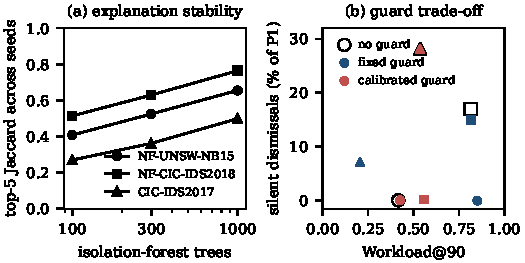
\includegraphics[width=\columnwidth]{figures/fig_results.pdf}
\caption{(a) Retraining the detector changes its explanations; larger forests reduce but do not remove the effect. (b) Workload against silent dismissals of P1 events for no guard (hollow), the fixed guard, and the calibrated guard; marker shape gives the corpus as in (a). Lower left is better; no guard setting is best on all corpora.}
\label{fig:results}
\end{figure}

\emph{Reproducibility of explanations (L2).} An explanation is a property of one trained model, not of the method: detectors that differ only in their seed explain the same alert with largely different features. An expert who quotes the top features of an alert must therefore show that they come from the model that made the decision. \textsc{XTriage} stores the content hashes of the detector and background set with every record and replays decisions exactly, so the quoted explanation stays verifiable. Larger forests reduce the disagreement (Fig.~\ref{fig:results}a) but do not remove it.

\emph{Anti-forensic steering (L4).} On CIC-IDS2017, moving attack traffic from port 80 to 443 leaves the score unchanged but changes the fired rule for 78\% of attack alerts and the tier for 36\%, so an attacker who knows the rules could lower an event's priority without looking less anomalous. Removing port bins from $\mathbf{z}$ removes the effect on all corpora at no cost. Restricting rules to SHAP-relevant features only moves the weakness: timing changes then downgrade 54\% of P1 events on NF-UNSW-NB15.

\emph{Known error rate (L5).} The silent dismissal rate is the error a reviewer or court would ask about, and Fig.~\ref{fig:results}b shows that no guard is best everywhere. The fixed guard is the safe default when attack classes shift between windows (CIC-IDS2017). The calibrated guard is far better when tune and test windows hold the same severe classes (NF-CIC-IDS2018: 0.2\% silent dismissals at lower workload) but fails when they differ, since a table learned from past decisions cannot anticipate unseen classes; its threshold also has a cliff ($\tau=0.02$ catches 96\% of severe errors, $\tau=0.05$ only 1\%). The guard setting and its error rate must be documented with every deployment.

\emph{Validity across networks (L7, L1).} Rules learned on NF-UNSW-NB15 fail on NF-CIC-IDS2018: half of all flows become alerts and AUROC falls below chance, so a triage tool must be validated where it is used. No triage layer recovers what the detector misses: late NF-CIC-IDS2018 Bot and Infiltration traffic looks benign to it (recall 0.7\%), and injected label noise even \emph{improved} macro-F1 there (0.59 to 0.69 at $\eta=0.3$), a sign that these classes are not learnable from flow features.

% ---------------------------------------------------------------------------
\section{\textsc{XFT-Bench}}
\label{sec:bench}
For every test flow of each corpus, \textsc{XFT-Bench} contains the features and identifiers, the score and percentile, SHAP values for three detector seeds and five hashed background sets (so stability can be studied without retraining), the fired rule, the guard status, the clean and noisy oracle priority, and the upstream label, together with the splits, rule sets, configuration, a datasheet \cite{gebru}, and regeneration scripts (144~MB of Parquet for the three corpora). Being derived from public corpora, it will be released under the upstream licences.

% ---------------------------------------------------------------------------
\section{Discussion and Threats to Validity}
\label{sec:discussion}
For forensic practice the results suggest four rules of use: record the model instance, background set, and rule set with every decision, since explanations are reproducible only for that combination; report the silent dismissal rate under the chosen guard setting as the tool's known error rate; keep attacker-controllable features such as ports out of triage rules; and validate the tool on the network where it is used. The rules, the guard, and the record make a decision defensible; the explanation alone does not.

Threats remain. The oracle only approximates investigators, who would use context such as asset value. The corpora are lab captures with known labelling errors \cite{engelen,sommer}, and we used the original CIC-IDS2017 labels. NetFlow lacks payloads, benign subsampling changes the base rate, the slow explainers ran on samples, and the probes use fewer seeds than the main comparison.

% ---------------------------------------------------------------------------
\section{Conclusion}
\label{sec:conclusion}
\textsc{XTriage} turns anomaly alerts into prioritized, explained, and replayable triage decisions. On three corpora it ranks severe events above score-only triage, makes every decision reconstructable and tamper-evident, and, with its guard, reduces severe events dismissed without warning. Its explanations, however, are reproducible only for the exact model instance; its rules can be steered by attackers through features the detector ignores; its error rate depends on a configurable guard; and it does not transfer between networks. Future work will make the autoencoder the primary detector, replace the oracle with real investigator decisions, and extend \textsc{XFT-Bench} to further corpora.

\begin{thebibliography}{00}
\bibitem{rogers} M. K. Rogers, J. Goldman, R. Mislan, T. Wedge, and S. Debrota, ``Computer forensics field triage process model,'' \emph{J. Digit. Forensics, Secur. Law}, vol. 1, no. 2, pp. 19--38, 2006.
\bibitem{nist} K. Kent, S. Chevalier, T. Grance, and H. Dang, ``Guide to integrating forensic techniques into incident response,'' NIST SP 800-86, 2006.
\bibitem{iso27037} \emph{Information Technology---Security Techniques---Guidelines for Identification, Collection, Acquisition and Preservation of Digital Evidence}, ISO/IEC 27037:2012, 2012.
\bibitem{iso27042} \emph{Information Technology---Security Techniques---Guidelines for the Analysis and Interpretation of Digital Evidence}, ISO/IEC 27042:2015, 2015.
\bibitem{daubert} \emph{Daubert v. Merrell Dow Pharmaceuticals, Inc.}, 509 U.S. 579, 1993.
\bibitem{iforest} F. T. Liu, K. M. Ting, and Z.-H. Zhou, ``Isolation forest,'' in \emph{Proc. IEEE ICDM}, 2008, pp. 413--422.
\bibitem{kitsune} Y. Mirsky, T. Doitshman, Y. Elovici, and A. Shabtai, ``Kitsune: An ensemble of autoencoders for online network intrusion detection,'' in \emph{Proc. NDSS}, 2018.
\bibitem{alahmadi} B. A. Alahmadi, L. Axon, and I. Martinovic, ``99\% false positives: A qualitative study of SOC analysts' perspectives on security alarms,'' in \emph{Proc. USENIX Security}, 2022.
\bibitem{sommer} R. Sommer and V. Paxson, ``Outside the closed world: On using machine learning for network intrusion detection,'' in \emph{Proc. IEEE S\&P}, 2010, pp. 305--316.
\bibitem{engelen} G. Engelen, V. Rimmer, and W. Joosen, ``Troubleshooting an intrusion detection dataset: The CICIDS2017 case study,'' in \emph{Proc. IEEE SPW}, 2021, pp. 7--12.
\bibitem{trustee} A. S. Jacobs \emph{et al.}, ``AI/ML for network security: The emperor has no clothes,'' in \emph{Proc. ACM CCS}, 2022.
\bibitem{arp} D. Arp \emph{et al.}, ``Dos and don'ts of machine learning in computer security,'' in \emph{Proc. USENIX Security}, 2022.
\bibitem{shap} S. M. Lundberg and S.-I. Lee, ``A unified approach to interpreting model predictions,'' in \emph{Adv. Neural Inf. Process. Syst.}, vol. 30, 2017.
\bibitem{warnecke} A. Warnecke, D. Arp, C. Wressnegger, and K. Rieck, ``Evaluating explanation methods for deep learning in security,'' in \emph{Proc. IEEE EuroS\&P}, 2020, pp. 158--174.
\bibitem{fooling} D. Slack, S. Hilgard, E. Jia, S. Singh, and H. Lakkaraju, ``Fooling LIME and SHAP: Adversarial attacks on post hoc explanation methods,'' in \emph{Proc. AAAI/ACM AIES}, 2020, pp. 180--186.
\bibitem{xgboost} T. Chen and C. Guestrin, ``XGBoost: A scalable tree boosting system,'' in \emph{Proc. ACM KDD}, 2016, pp. 785--794.
\bibitem{treeshap} S. M. Lundberg \emph{et al.}, ``From local explanations to global understanding with explainable AI for trees,'' \emph{Nat. Mach. Intell.}, vol. 2, pp. 56--67, 2020.
\bibitem{lime} M. T. Ribeiro, S. Singh, and C. Guestrin, ```Why should I trust you?': Explaining the predictions of any classifier,'' in \emph{Proc. ACM KDD}, 2016, pp. 1135--1144.
\bibitem{hermosilla} P. Hermosilla, S. Berr\'ios, and H. Allende-Cid, ``Explainable AI for forensic analysis: A comparative study of SHAP and LIME in intrusion detection models,'' \emph{Appl. Sci.}, vol. 15, no. 13, Art. no. 7329, 2025.
\bibitem{ripper} W. W. Cohen, ``Fast effective rule induction,'' in \emph{Proc. ICML}, 1995, pp. 115--123.
\bibitem{anchors} M. T. Ribeiro, S. Singh, and C. Guestrin, ``Anchors: High-precision model-agnostic explanations,'' in \emph{Proc. AAAI}, 2018.
\bibitem{adewole} K. S. Adewole, A. Jacobsson, and P. Davidsson, ``Intrusion detection framework for Internet of Things with rule induction for model explanation,'' \emph{Sensors}, vol. 25, no. 6, Art. no. 1845, 2025.
\bibitem{rudin} C. Rudin, ``Stop explaining black box machine learning models for high stakes decisions and use interpretable models instead,'' \emph{Nat. Mach. Intell.}, vol. 1, pp. 206--215, 2019.
\bibitem{unsw} N. Moustafa and J. Slay, ``UNSW-NB15: A comprehensive data set for network intrusion detection systems,'' in \emph{Proc. MilCIS}, 2015.
\bibitem{cicids} I. Sharafaldin, A. H. Lashkari, and A. A. Ghorbani, ``Toward generating a new intrusion detection dataset and intrusion traffic characterization,'' in \emph{Proc. ICISSP}, 2018, pp. 108--116.
\bibitem{maseno} E. M. Maseno, Y. Sun, and Z. Wang, ``Reliability auditing of explanations for machine-learning-based intrusion detection systems,'' \emph{J. Comput. Virol. Hacking Tech.}, vol. 22, Art. no. 80, 2026.
\bibitem{gombar} M. Gombar, ``From detection to triage: Explainable suspicious flow prioritization for multiclass intrusion detection using CSE-CIC-IDS2018,'' \emph{Electronics}, vol. 15, no. 12, Art. no. 2739, 2026.
\bibitem{nfv3} University of Queensland, ``NetFlow v3 datasets,'' [Online]. Available: https://staff.itee.uq.edu.au/marius/NIDS\_datasets/, accessed Oct. 2026.
\bibitem{brodley} C. E. Brodley and M. A. Friedl, ``Identifying mislabeled training data,'' \emph{J. Artif. Intell. Res.}, vol. 11, pp. 131--167, 1999.
\bibitem{gebru} T. Gebru \emph{et al.}, ``Datasheets for datasets,'' \emph{Commun. ACM}, vol. 64, no. 12, pp. 86--92, 2021.
\bibitem{gridsoc} D. Popoola, S. Bhattacharya, A. Hahn, and M. Govindarasu, ``AI-enabled security operations center (SOC) for modern power grids: Bridging the gap between the cybersecurity and grid operations,'' \emph{IEEE Power Energy Mag.}, pp. 57--69, Sep./Oct. 2026, doi: 10.1109/MPE.2026.3705348.
\bibitem{cysider} D. Popoola, S. Bhattacharya, and M. Govindarasu, ``CySIDER: Cybersecurity situational intelligence framework for DER networks,'' in \emph{Proc. Resilience Week (RWS)}, National Harbor, MD, USA, 2025, pp. 1--10, doi: 10.1109/RWS66711.2025.11304446.
\bibitem{excyder} D. Popoola, S. Bhattacharya, and M. Govindarasu, ``Self-verifying anomaly detection using explainable AI for cybersecurity of DER networks,'' in \emph{Proc. IEEE PES General Meeting (PESGM)}, 2026.
\bibitem{cytrex} D. Popoola, S. Bhattacharya, and M. Govindarasu, ``CyTReX: Explainable AI-based cybersecurity threat reasoning framework for DER networks,'' presented at \emph{Resilience Week (RWS)}, National Harbor, MD, USA, 2026, arXiv:2610.04286.
\end{thebibliography}

\end{document}
